\chapter{Progetto di \emph{stage}}
\label{cap:progettoDiStage}

\section{Visione aziendale}
\subsection{Rapporto dell'azienda con gli \emph{stage}}
Wintech identifica gli \emph{stage} universitari come strumenti utili alla formazione professionale dei laureandi al fine di renderli risorse produttive non solo per il periodo di \emph{stage} definito, ma soprattutto per il periodo successivo. È infatti consuetudine per l'azienda decidere di proseguire i rapporti lavorativi con gli studenti, pertanto, è nel suo interesse rendersi disponibile fornendo approfondimenti e attività formative in ambito tecnologico e riguardo i processi aziendali.\\
Per proporre la propria disponibilità e avere un primo contatto con gli studenti, Wintech partecipa da diversi anni all'evento dedicato STAGE-IT promosso da Confindustria Veneto Est in collaborazione con i Dipartimenti di Scienze Statistiche, Matematica e Ingegneria dell'Informazione dell'Università di Padova, al fine di favorire l'incontro tra aziende associate e gli studenti per esporre i progetti \gls{ICT} proposti.\\
Successivamente, organizza colloqui conoscitivi al fine di spiegare la propria visione aziendale e i propri progetti di \emph{stage} agli studenti.\\
Essi non sono pensati per essere esclusivamente didattici ma forniscono un tangibile valore all'azienda in quanto si basano sulle tecnologie e metodologie da loro realmente utilizzate o che prevedono di integrare.\\
Lo stagista non è pertanto visto solo come uno studente ma viene integrato nel \emph{team} con il quale lavora a stretto contatto acquisendo nuove competenze sia collaborativamente, mediante meeting e sviluppo cooperativo, che autonomamente, mediante fasi di ricerca e sviluppo individuali.\\

\subsection{Progetti proposti}
I progetti di \emph{stage} proposti dall'azienda, contestualmente al periodo della nostra collaborazione, derivano dal valore aggiunto che l'automazione dei processi aziendali può portare in ambiti di pianificazione progettuale, per ambienti di sviluppo consolidati e per tecnologie oggetto di ricerca.\\
Tale processo permette di realizzare efficientemente prodotti con maggiore qualità riducendo sensibilmente i tempi e i costi dei lavori.\\
Inoltre, automatizzare attività ben definite riduce sensibilmente la possibilità di introduzione manuale di errori e ne permette una rapida individuazione.\\
Durante la durata dello \emph{stage}, noi stagisti abbiamo collaborato più volte trovando dei punti di incontro tra i propri progetti e rimanendo aggiornati riguardo ai rispettivi risultati ottenuti tramite appositi incontri.\\
I tre progetti proposti in questione sono: 

\subsubsection*{Applicativi di DevOps in ambito Sistemi e Office365}
\label{mioStage}
Lo scopo dello \emph{stage} da me svolto è stato quello di compiere un'analisi per verificare l'applicabilità delle pratiche di \gls{DevOps} su progetti basati sull'utilizzo di tecnologie Office365, con lo scopo di integrarle nell'infrastruttura aziendale in maniera rapida e \emph{low-code}, ovvero con limitata necessità e presenza di codice scritto dallo sviluppatore. Più specificatamente sono stati utilizzati i programmi Power Automate e Power Apps: il primo permette di realizzare flussi di attività connesse con gli applicativi Microsoft, mentre il secondo agevola lo sviluppo di applicazioni aziendali.\\
Le soluzioni individuate durante la ricerca vengono introdotte nel contesto aziendale tramite fasi di sviluppo sia implementando tali risultati a reali applicazioni aziendali, realizzate collaborando con il \emph{team}, sia producendo \emph{Proof of Concept} (PoC), ovvero elementi dimostrativi sviluppati al fine di provare la fattibilità di un prodotto mediante l'utilizzo delle tecnologie e degli strumenti definiti. Esso rappresenta quindi una versione di prova prototipale e non ha lo scopo di divenire il prodotto finale ma viene realizzato a supporto dell'analisi progettuale.
\begin{figure}[htbp] 
    \centering 
    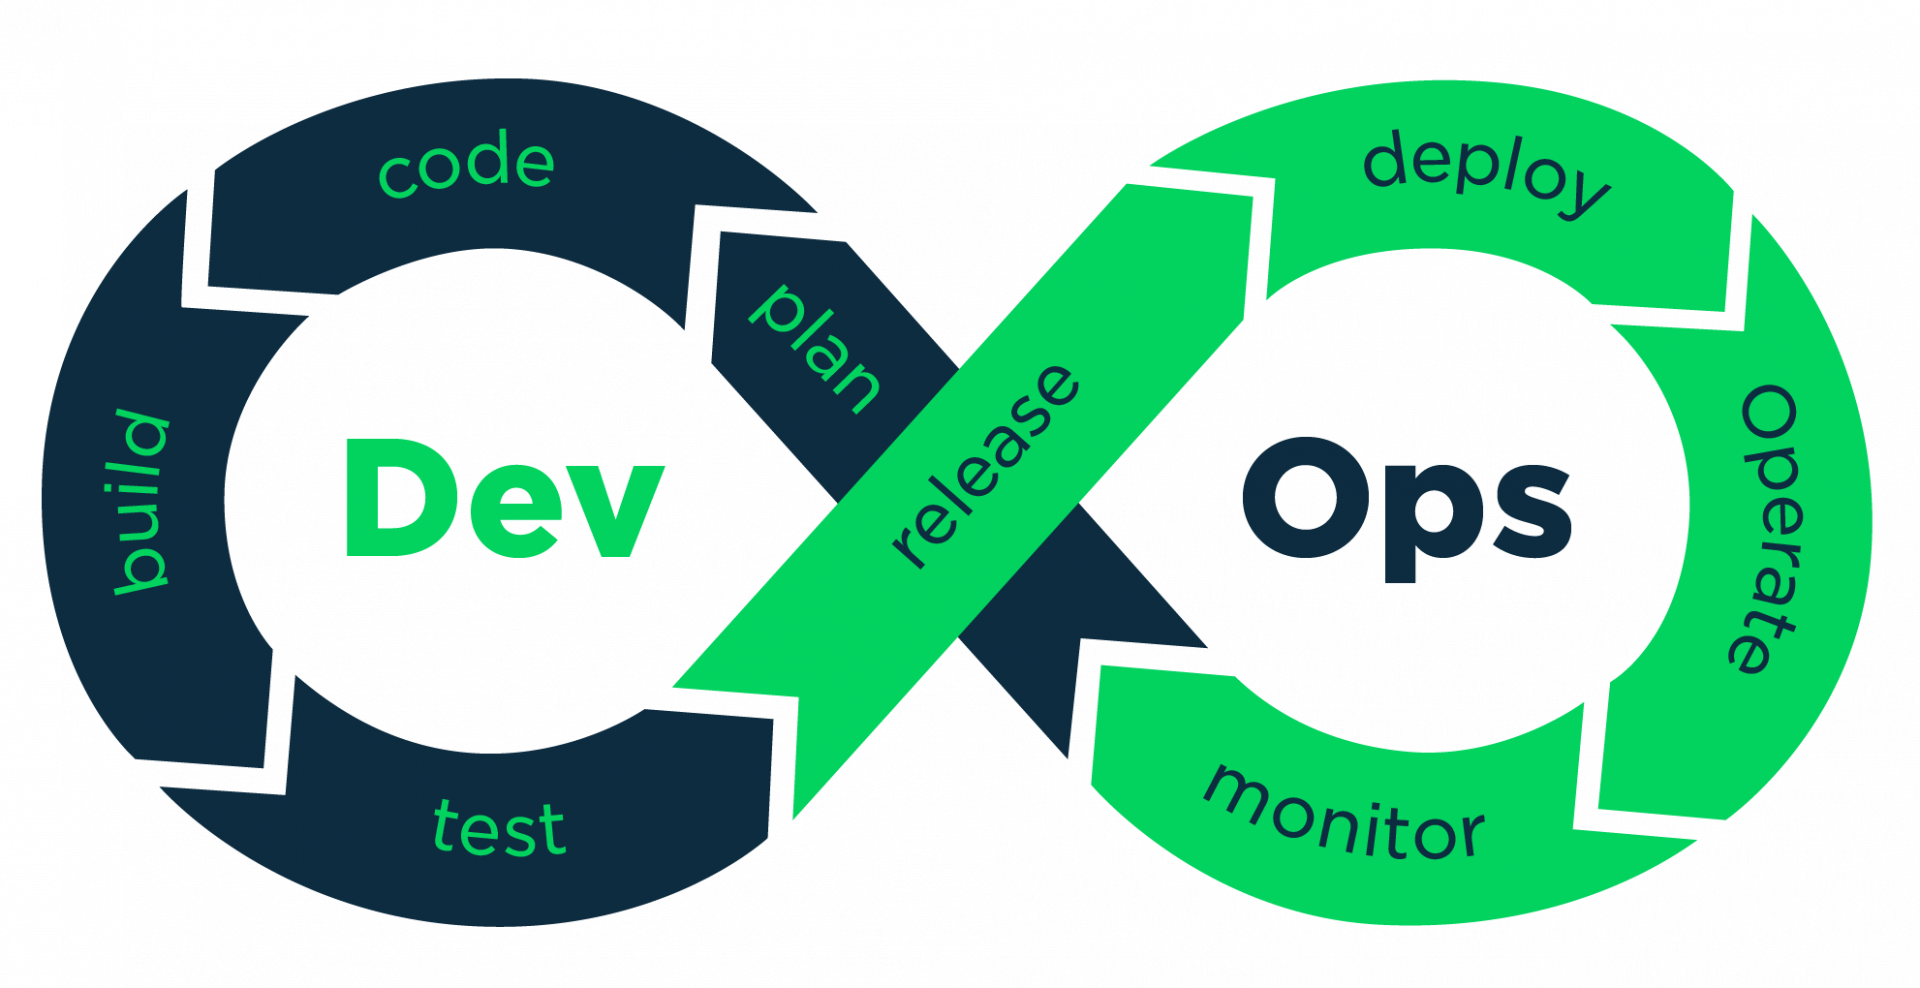
\includegraphics[width=0.8\columnwidth]{DevOps}
    \caption{Ciclo e fasi di DevOps.} 
    \label{fig:DevOps}
\end{figure}

\subsubsection*{Integrazione sistemi di pianificazione di progetto}
Lo scopo dello \emph{stage} è stado compiere un'analisi per verificare l'utilizzo degli strumenti di pianificazione aziendale, nello specifico Planner e Taiga, e lo sviluppo di una soluzione atta ad automatizzare la comunicazione e sincronizzazione di tali strumenti.\\
Per raggiungere tale obiettivo è stato possibile utilizzare le \emph{Application Programming Interface} (API): in italiano "Interfacce di Programmazione dell'Applicazione". Esse rappresentano un insieme di procedure che permettono la comunicazione e lo scambio di dati tra diversi componenti \emph{software}. L'utilizzo di API permette di semplificare l'integrazione tra prodotti e servizi informatici rendendo disponibili funzionalità esterne senza doverne conoscere l'effettiva implementazione.

\subsubsection*{Applicativi di DevOps in ambito Sistemi}
\label{stageDavide}
Lo scopo dello \emph{stage} è stato compiere un'analisi per verificare l'applicabilità delle pratiche di \gls{DevOps} all'ambiente di sviluppo \gls{Sistemi}, con lo scopo di integrarle nell'infrastruttura aziendale in ambiti ben definiti.\\
Le soluzioni individuate durante la ricerca vengono introdotte nel contesto aziendale tramite fasi di sviluppo. 


\section{\emph{Stage} da me svolto}
%\hyperref[mioStage]{Applicativi di DevOps in ambito Sistemi e Office365}
\subsection{Obiettivi progettuali}
Gli obiettivi attesi del mio \emph{stage} esprimono la necessità di uno studio approfondito riguardo all'ambiente Office365 e più specificatamente delle tecnologie Power Automate e Power Apps.\\
Tale studio deve essere accompagnato da fasi di sviluppo al fine di integrare e testare le soluzioni individuate durante la ricerca.\\
Ogni conclusione raggiunta deve essere opportunamente documentata in modo da definire se e come le metodologie \gls{DevOps} aziendali siano applicabili all'ambiente Office365. Al \emph{team} di sviluppo e al \emph{tutor} aziendale dovranno essere esposte delle presentazioni relative a quanto appreso.\\
Rientra tra gli obiettivi comprendere l'importanza e l'impatto che l'automazione possiede quando applicata correttamente ai processi lavorativi e comprendere le potenzialità delle metodologie DevOps e delle tecnologie in oggetto.
Sono previsti tra gli obiettivi di \emph{stage} anche delle fasi di sviluppo in collaborazione con il team dell'unità operativa ricerca e sviluppo, al fine di comprendere e migliorare prodotti aziendali realizzati utilizzando le tecnologie in oggetto. I documenti di sviluppo sicuro relativi ai progetti realizzati precedentemente allo \emph{stage} devono essere adattati in caso di modifiche al \emph{software} o alle metodologie applicate.
La scelta di assegnare all'unità operativa Ricerca e sviluppo lo studio e l'utilizzo delle tecnologie Power Automate e Power apps deriva dal bisogno di identificare un nuovo metodo che permetta di risparmiare tempo nelle fasi di sviluppo senza rinunciare alla qualità dei prodotti.\\
Esse, avendo una natura \emph{low-code} ed essendo pensate per fornire nativamente un'agevole connessione con gli altri servizi Microsoft, permettono di applicare le personalizzazioni richieste da un cliente in maniera più rapida e sicura rispetto allo sviluppo delle stesse soluzioni tramite linguaggi di programmazione e altri strumenti consolidati.\\
È quindi mio obiettivo fondamentale verificare l'idoneità di tali strumenti al soddisfacimento del bisogno descritto.
L'ultimo obiettivo espresso dall'azienda è la realizzazione di una presentazione finale collaborativamente tra i tre stagisti al termine dei loro periodi di \emph{stage} e la sua esposizione al presidente di Wintech e ai responsabili.\\\\

\subsection{Vincoli temporali}
Lo \emph{stage} ha avuto inizio il giorno 11 settembre ed è terminato il giorno 20 novembre.\\
Esso ha avuto luogo interamente in presenza nella sede di Padova, nella quale mi sono recato dalle ore 9:00 alle ore 13:00 e dalle ore 14:00 alle ore 18:00, per un totale di 320 ore lavorative.\\
Tale periodo è stato suddiviso in otto fasi pianificate ben definite, come dichiarato nel documento “Progetto Formativo”, fornitomi dal \emph{tutor} aziendaele, generato all'inizio dello stage:
\subsubsection*{Fase 1: dal 11/09/2024 al 13/09/2024 (24h)}
Lo studente insieme agli \emph{stakeholder} prende confidenza con l'ambito di riferimento per lo \emph{stage} e visiona come il ciclo di vita del \emph{software} e le metodologie \gls{DevOps} siano state applicate in azienda con lo sviluppo sicuro.\\
Lo studente analizza le funzionalità di versionamento con Git e Git Server.\\

\subsubsection*{Fase 2: dal 16/09/2024 al 20/09/2024 (40h) }
Lo studente utilizza le funzionalità di versionamento con Git e il Git Server fornito dall'azienda per versionare il modulo di riferimento, eseguire delle modifiche per dimostrare: salvataggio, modifiche, autori e date, \emph{blame}, \emph{branch}, \emph{merge}, \emph{tag}.\\
Lo studente determina insieme ai \emph{developer} dell'ambito di riferimento se è possibile versionare agevolmente con gli strumenti a disposizione e che differenze ci sono nell'ambito specifico preso a riferimento: \gls{Sistemi}.\\
Lo studente compila con i \emph{developer} il documento di \gls{DevOps} di sviluppo sicuro.\\

\subsubsection*{Fase 3: dal 07/10/2024 al 11/10/2024 (40h) }
Lo studente fornisce i suoi \emph{feedback} su quanto appreso e sponsorizza la sua esperienza ai \emph{team} realizzando documentazione e presentazione.\\

\subsubsection*{Fase 4: dal 14/10/2024 al 18/10/2024 (40h) }
Lo studente valuta se sia possibile utilizzare IDE non proprietari in ambito \gls{Sistemi}. Tale acronimo indica il termine \emph{Integrated Development Environment} (ambiente di sviluppo integrato), ovvero un'applicazione che permette di sviluppare codice sorgente in una moltitudine di diversi linguaggi di programmazione e può fornire servizi come \emph{testing}, analisi statica del codice, \emph{debugging}, compilazione e integrazione con sistemi di versionamento.\\ 
In seguito viene valutata la possibilità di utilizzare lo strumento di analisi statica SonarLint negli IDE in ambito \gls{Sistemi} o altri strumenti similari utilizzando come guida i documenti di sviluppo sicuro.\\
Lo studente riporta le considerazioni in documentazione ed esegue una presentazione agli \emph{stakeholder}.\\ 
\begin{figure}[htbp] 
    \centering 
    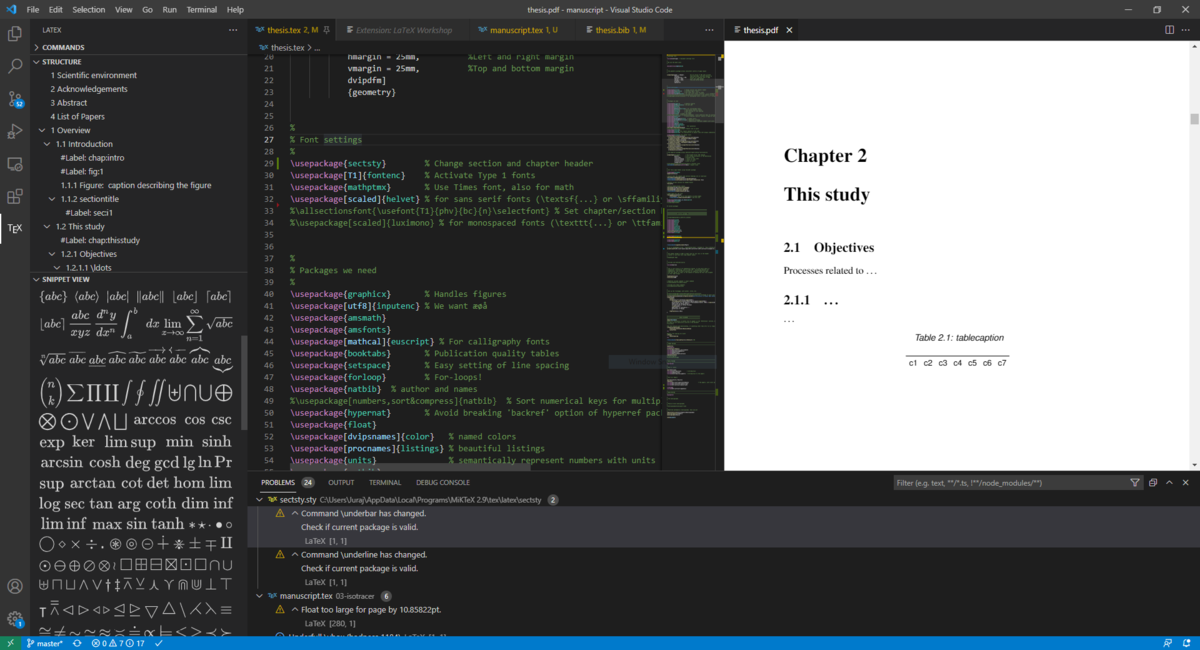
\includegraphics[width=1\columnwidth]{esempioVSCode}
    \caption{Interfaccia grafica di esempio dell'IDE Visual Studio Code.} 
    \label{fig:esempioVSCode}
    \vspace{1mm}
    Fonte: \url{https://commons.wikimedia.org/wiki/File:VsCode_LaTex_Workshop.png}.
\end{figure}
\subsubsection*{Fase 5: dal 21/10/2024 al 25/10/2024 (40h) }
Lo studente discutere con gli \emph{stakeholder} come viene utilizzato Jenkins e come è stato sponsorizzato e analizzato nei documenti di sviluppo sicuro, prende confidenza con Jenkins realizzando un \emph{job} che compila un modulo di esempio. Lo studente determina se sia stato possibile compilare in ambito \gls{Sistemi} con l'\emph{automation server} Jenkins come descritto nei documenti di sviluppo sicuro.\\

\subsubsection*{Fase 6: dal 28/10/2024 al 31/10/2024 e dal 04/11/2024 al 08/11/2024 (72h)}
Lo studente insieme ai colleghi inserisce dei \emph{test} di esempio verificando di poterli eseguire con Jenkins e ne visiona i \emph{report}.\\
Verifica le possibilità di \emph{deploy} tramite Jenkins. Verifica come sia composto il \emph{server} in cui eseguire il \emph{deploy} schematizzando le sue parti insieme ai colleghi.\\

\subsubsection*{Fase 7: dal 11/11/2024 al 15/11/2024 (40h) }
Lo studente fornisce i suoi \emph{feedback} finali su quanto appreso tramite l'\emph{automation server} e sponsorizza la sua esperienza ai \emph{team} realizzando documentazione e presentazione.\\

\subsubsection*{Fase 8: dal 18/11/2024 al 20/11/2024 (24h) }
Lo studente interpreta l'esperienza per discutere dei vantaggi nell'uso di un sistema di \emph{build} e \emph{deploy} automatizzato. Ogni esperienza fatta durate lo \emph{stage} è corredata da documentazione, versionamento di configurazioni o \emph{software} se utilizzati.\\
Viene eseguita una presentazione finale.\\
\begin{figure}[htbp] 
    \centering 
    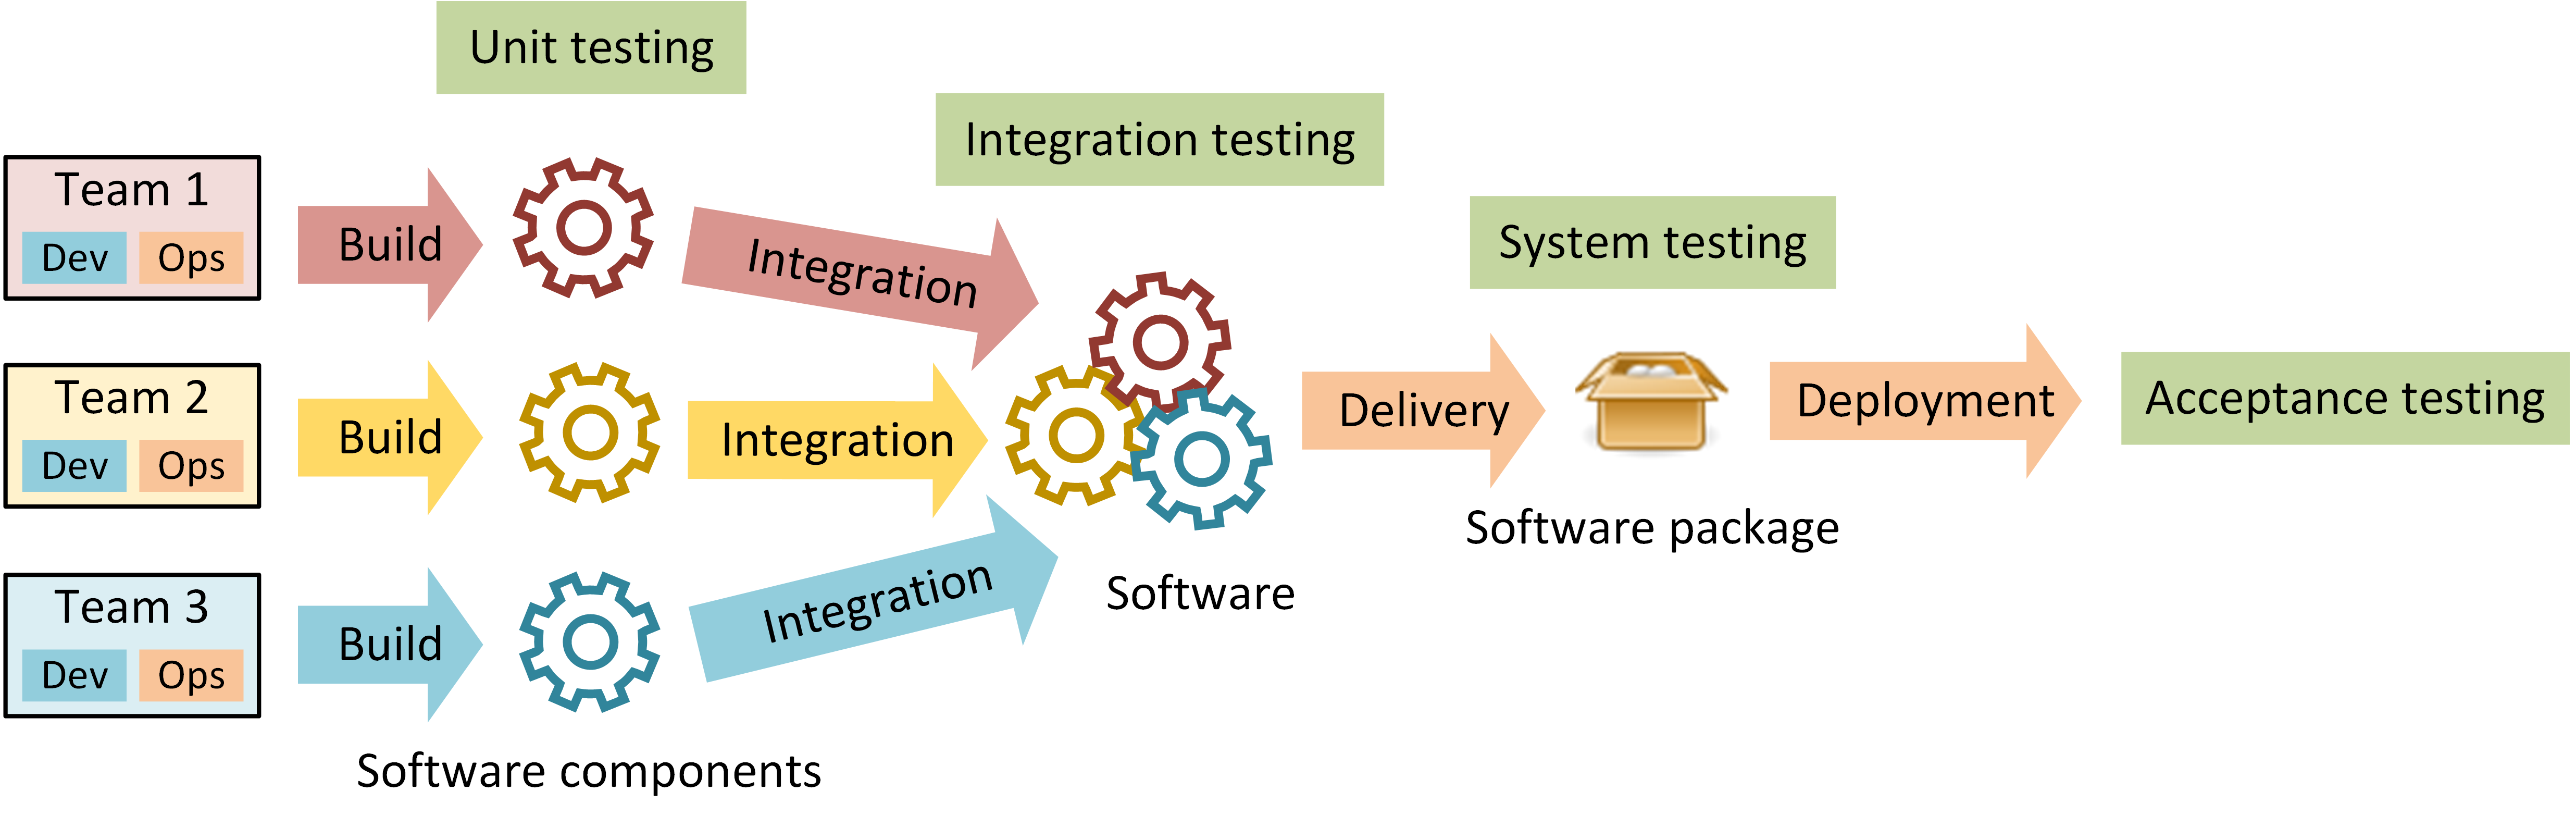
\includegraphics[width=1\columnwidth]{buildToDeployment}
    \caption{Flusso di Build, Delivery e Deployment in ambito DevOps.} 
    \label{fig:buildToDeployment}
    \vspace{1mm}
    Fonte: \url{https://commons.wikimedia.org/wiki/File:DevOps_from_Integration_to_Deployment.png}.
\end{figure}
\newline \newline \noindent Tali indicazioni sono state intese come delle linee guida e non come dei vincoli ferrei, pertanto, ho avuto la libertà di autogestire le mie attività dando priorità alle necessità e alle direttive fornitemi con l'avanzamento dei lavori.\\
Esse hanno rispettato quanto descritto con la differenza che è stata data maggiore importanza all'applicazione delle fasi di \gls{DevOps} in ambienti Office365 e allo sviluppo con le tecnologie Power Automate e Power Apps.\\
Inizialmente era incluso fortemente l'ambiente \gls{Sistemi} nelle fasi del progetto poiché era prevista una maggiore collaborazione con lo stage \hyperref[stageDavide]{Applicativi di \gls{DevOps} in ambito Sistemi}.\\
Questi riallineamenti sono avvenuti in maniera naturale e coerentemente con le necessità e indicazioni fornitemi dal \emph{tutor} aziendale.\\
Durante l'avanzamento dei lavori, le attività da me svolte sono sempre state dichiarate tramite lo strumento Planner, inoltre tutti i documenti da me realizzati sono stati condivisi in un ambiente comune al fine di mantenere chiarezza con il \emph{team} e il \emph{tutor} aziendale.\\
Con quest'ultimo ho avuto uno stretto contatto durante il periodo di \emph{stage} in modo da favorire l'interazione e garantire il raggiungimento degli obiettivi prefissati.\\
Ad ogni significativo risultato ottenuto ho realizzato la relativa documentazione e una presentazione successivamente esposta al \emph{tutor} e al \emph{team} di sviluppo.\\

\subsection{Obiettivi personali}
Durante l'evento STAGE-IT avvenuto il giorno 8 aprile 2024, ho potuto dialogare con diverse aziende relativamente ai loro progetti di \emph{stage} offerti. Sono seguitati colloqui nelle rispettive sedi e infine ho convenuto che l'azienda che mi suscitava maggiore interesse fosse Wintech.\\
Questo è conseguenza dell'organizzazione aziendale in linea con i processi studiati durante il corso di studi, l'attenzione che è stata posta fin da subito agli stagisti e all'innovazione e grazie ai progetti di \emph{stage} relativi a tematiche di mio interesse.\\
È per tali motivazioni che i miei obiettivi personali sono stati:
\begin{itemize}
    \item Introduzione ad un contesto lavorativo, legato al percorso di studi da me frequentato, che comprendesse i principali processi aziendali studiati. 
    \item Collaborazione con un \emph{team} di sviluppo professionale utilizzando gli strumenti adeguati. 
    \item Sviluppo, analisi ed integrazione con il contesto aziendale di tecnologie per me nuove. Creazione della conseguente adeguata documentazione. 
    \item Realizzazione di flussi di automazione in grado di migliorare la produttività e la qualità dei processi aziendali e di aggiungere importanti funzionalità ad applicazioni e prodotti reali. 
    \item Gestione delle risorse e del tempo fornitomi per organizzare e realizzare in autonomia i \emph{task} definiti in fase di pianificazione.\\
\end{itemize}
È stato nel mio interesse entrare in un contesto lavorativo al fine di crescere professionalmente e acquisire maggiori opportunità in vista del periodo successivo al conseguimento della laurea. 
 
 
